%%%%%%%%%%%%%%%%%%%%%%%%%%%%%%%%%%%%%%%%%
% Stylish Article
% LaTeX Template
% Version 2.2 (2020-10-22)
%
% License:
% CC BY-NC-SA 3.0 (http://creativecommons.org/licenses/by-nc-sa/3.0/)
%
%%%%%%%%%%%%%%%%%%%%%%%%%%%%%%%%%%%%%%%%%

%----------------------------------------------------------------------------------------
%	PACKAGES AND OTHER DOCUMENT CONFIGURATIONS
%----------------------------------------------------------------------------------------

\documentclass[fleqn, 11pt]{SelfArx} % Document font size and equations flushed left

\usepackage[english]{babel} % Specify a different language here - english by default

\usepackage{lipsum} % Required to insert dummy text. To be removed otherwise

\usepackage{array} % Required for centering tables content

\usepackage{float} % Avoid putting tables on top of the pages

\graphicspath{ {./images/} } % Paths were images are taken

%----------------------------------------------------------------------------------------
%	COLUMNS
%----------------------------------------------------------------------------------------

\setlength{\columnsep}{0.55cm} % Distance between the two columns of text
\setlength{\fboxrule}{0.75pt} % Width of the border around the abstract

%----------------------------------------------------------------------------------------
%	COLORS
%----------------------------------------------------------------------------------------

\definecolor{color1}{RGB}{0,0,90} % Color of the article title and sections
\definecolor{color2}{RGB}{0,20,20} % Color of the boxes behind the abstract and headings

%----------------------------------------------------------------------------------------
%	HYPERLINKS
%----------------------------------------------------------------------------------------

\usepackage{hyperref} % Required for hyperlinks

\hypersetup{
	hidelinks,
	colorlinks,
	breaklinks=true,
	urlcolor=color2,
	citecolor=color1,
	linkcolor=color1,
	bookmarksopen=false,
	pdftitle={Title},
	pdfauthor={Author},
}

\setlength{\parindent}{0cm} % Remove left padding from text

\newcolumntype{C}[1]{>{\centering\arraybackslash}p{#1}} % centering columns values

%----------------------------------------------------------------------------------------
%	ARTICLE INFORMATION
%----------------------------------------------------------------------------------------

\JournalInfo{\today} % Journal information
\Archive{\textcopyright \space 2022} % Additional notes (e.g. copyright, DOI, review/research article)

\PaperTitle{Implementation of DoS attack through mDNS and brief discussion on its vulnerabilities} % Article title

\Authors{A. Al Masoud • F. Amato • A. Blindu • D. Lotito • D. Ragusa} % Authors
\affiliation{\textit{Department of Computer Engineering, University of Pavia, Pavia, Italy}} % Author affiliation
\affiliation{\textit{Enterprise Digital Infrastructure}} % Author affiliation

\Keywords{\small{DoS • mDNS • Security • LAN }} % Keywords - if you don't want any simply remove all the text between the curly brackets
\newcommand{\keywordname}{Keywords} % Defines the keywords heading name

%----------------------------------------------------------------------------------------
%	ABSTRACT
%----------------------------------------------------------------------------------------

\Abstract{The aim of this report is to study and discuss the implementation of a DoS attack on a local network exploiting the mDNS protocol. 
The traffic that was generated has been analyzed and some studies have been conducted
in order to understand the impact of this kind of DoS attack under different conditions.
Moreover, other possible vulnerabilities of this protocol have been studied with their countermeasure to understand their possible effect.}

%----------------------------------------------------------------------------------------

\begin{document}

\maketitle % Output the title and abstract box

\tableofcontents % Output the contents section

\thispagestyle{empty} % Removes page numbering from the first page

%----------------------------------------------------------------------------------------
%	INTRODUCTION
%----------------------------------------------------------------------------------------

\section{Introduction} % The \section*{} command stops section numbering
The idea behind this project is to implement a DoS attack exploiting the mDNS (Multicast Domain Name System) protocol \cite{rfc6762} on a local area network which could use it to make various IoT devices communicate, this to show how easily inaccessible the service can be made. \newline

In general, a DoS attack is when an attacker is attempting to make it impossible for a target service, or multiple services, to operate properly. These attacks work by overwhelming a system with requests for data. \newline
This goal is usually achieved by sending small requests to a third party service, spoofing the IP address of the target one, and this third party service in turn respond with bigger response to the target letting it to crash. \newline The result is that available internet bandwidth and the resources of the target system become overloaded.\newline
In this project, the mDNS protocol was used because it would allow amplification by exploiting particular types of queries that send a lot of data (ANY type) and also reflection, sending packets to all devices in the network through multicast mode. \newline

To simplify the work and avoid legal problems, the initial assumption was that the attacker and the target devices are within the same network although, as will be explained below, the striker could also act from the outside in case of misconfiguration.

%----------------------------------------------------------------------------------------
%	mDNS protocol
%----------------------------------------------------------------------------------------

\section{The mDNS protocol}
Multicast DNS (mDNS) is a service that aims to solve name resolution in smaller networks. It takes a different approach than the well-known DNS: instead of sending requests to a name server, the network participants are all contacted through multicast mode. \newline
Instead, a similarity to the classic DNS protocol is that mDNS is an application layer protocol if TCP/IP network stack is considered. \newline % so in this case the communication stack is the one displayes in \ref{fig:stack}. \newline

% \begin{figure}[H]\centering
%     \includegraphics[width=\linewidth]{stack.png}
%     \caption{TCP/IP Network Stack}
%     \label{fig:stack}
% \end{figure}

A client, that needs to know information about an hostname, sends a query to all the devices in the network. The response, instead, should go to the entire network or directly to the client in unicast. In this way, if the answer is sent to all devices in multicast, all of them are informed about the name and IP address such that they can create an entry in their mDNS cache. \newline
Multicast DNS can cause relatively high traffic, so the protocol actively tries to conserve network resources: to this end, the requesting client sends the correct response according to its opinion (i.e. according to the current cache entry). Only if this is no longer correct, or if the entry is about to expire, the recipient have to respond. \newline

Generally, only hostnames ending with {\it{.local}} can be used with Multicast DNS. Another characteristic is that it relies on top of the UDP protocol at the transport layer.\newline

\begin{figure}[H]\centering
    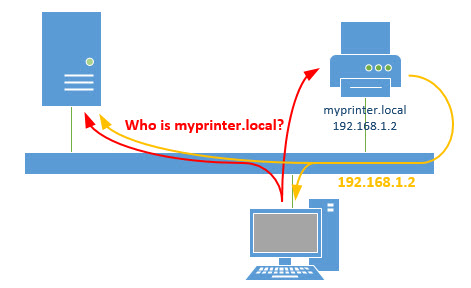
\includegraphics[width=\linewidth]{./mdns-02.jpg}
    \caption{Example of mDNS operation where the query (red) is sent to all devices and the same happens for the response (yellow) from the printer}
    \label{fig:msdns-1}
\end{figure}

The mDNS was developed in the context of Zeroconf (Zero Configuration Networking) using essentially the same programming interfaces (packet formats) and operating semantics as the unicast Domain Name Service (DNS). The idea behind Zero Configuration Networking is to allow computers to communicate with each other without the need for a prior configuration.\newline

A popular implementation of mDNS is \textit{Bonjour} by Apple, but also the open source software \textit{Avahi} can be used as an mDNS service. As of Windows 10, mDNS is also available in Microsoft's operating system.

\paragraph{Advantages} 
\begin{itemize}[leftmargin=*]
    \item Since all devices share their IP addresses, there is no need to configure a server or directory. This makes it possible to add additional devices very dynamically and quickly.
\end{itemize}

\paragraph{Disadvantages} 
\begin{itemize}[leftmargin=*]
    \item One problem lies in the multicast procedure itself. Although the protocol tries to keep network traffic low, participating computers must constantly monitor the network and process incoming messages. This requires computing power.
    \item Assigning host names is problematic: since you can freely choose a name for each device, as long as it ends in {\it{.local}}, this can (at least theoretically) lead to two network devices with the same host name. The developers of mDNS have deliberately not proposed a solution to this problem: on the one hand, it is assumed that the case rarely occurs; on the other hand, the double naming may be intentional. \newline 
    Also, by default, mDNS only resolves hostnames that end with the {\it{.local}} top-level domain. This can cause problems if {\it{.local}} includes hosts that do not implement mDNS but can be found via a conventional unicast DNS server. Resolving such conflicts requires network configuration changes that mDNS is designed to avoid.
    \item In some cases, mDNS is open. This means that it also responds to requests from outside (the Internet). Attackers can find such open services and use them for DoS attacks, using network devices improperly. \newline
    In addition, using mDNS, even sensitive data can be detected. This allows attackers to know information about connected devices and use it for further attacks.
\end{itemize}

\subsection{Packets structure}
An mDNS message is a UDP packet sent in multicast using the following addressing:
\begin{itemize}[leftmargin=*]
    \item IPv4 address \textit{224.0.0.251} or IPv6 address \textit{ff02::fb}
    \item UDP port \textit{5353}
\end{itemize}
The payload structure is based on the unicast DNS packet format, which consists of two parts: the header and the data.\newline
The header, shown in Figure \ref{fig:msdns-message-1}, is identical to the one found in the unicast DNS, as are the subsections in the data part: queries, responses, authoritative-nameservers, and additional records.

\begin{figure}[H]\centering
    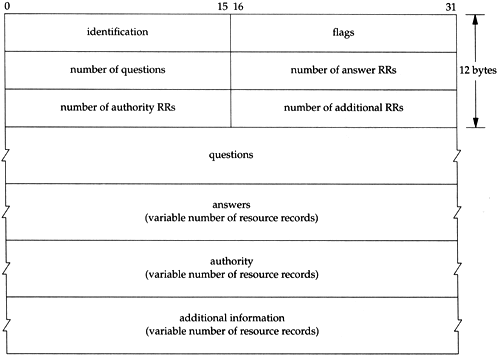
\includegraphics[width=\linewidth]{./msg-format.png}
    \caption{mDNS/Unicast DNS message format}
    \label{fig:msdns-message-1}
\end{figure}

\subsection{Queries}
The format, shown in Table \ref{tab:query-section}, of the query section is a bit different from that of the classic DNS because it adds a single-bit {\it{"QU" question}} field. \newline

\begin{table}[hbt]
	\centering
	\begin{tabular}{|C{2cm}|C{2.8cm}|C{1.5cm}|}
		\hline
		\textbf{Field} & \textbf{Description} & \textbf{Length} \\
		\hline
		\hline
		Name & Name of the node to which the query pertains & Variable \\
		\hline
		Type &	The type of the query &	16 \\
		\hline
		Class & IN & 15 \\
		\hline
		"QU" question & Boolean flag indicating whether a unicast response is desired & 1 (higher order bit of Class field)\\
		\hline
	\end{tabular}
	\caption{Query section fields}
	\label{tab:query-section}
\end{table}

The {\it{Class}} field is identical to that found in unicast DNS ({\it{IN}} class).
The {\it{"QU" question}} field is used to minimize unnecessary transmissions over the network: if the bit is set (the high order bit of the Class field), responders should send a direct-unicast response to the requesting node rather than broadcasting the response to the entire network.\newline

\subsection{Resource Records}
All records in the answers, authoritative-nameservers, and additional records sections have the same format while the RRs in the answer section in mDNS are slightly different from classic DNS. What they are and their length are shown in Table \ref{table}. \newline

In particular, the {\it{Cache-flush}} bit is used to instruct neighboring nodes that the record should overwrite, rather than be added to any existing cache entry for this RR {\it{Name}} and {\it{Type}}.

\begin{table}[hbt]
	\centering
	\begin{tabular}{|C{2.0cm}|C{4.2cm}|C{1.25cm}|}
		\hline
		\textbf{Field} & \textbf{Description} & \textbf{Length} \\
		\hline
		\hline
		Name & Name of the node to which the record pertains & Variable\\
		\hline
		Type & Type of the Resource Record & 16\\
		\hline
		Class & Class code, 1 a.k.a. IN for the Internet and IP networks & 15\\
		\hline
		Cache-flush & Boolean flag indicating whether outdated cached records should be purged & 1\\
		\hline
		TTL & Time interval (in seconds) that the RR should be cached & 32\\
		\hline
		Data length & Integer representing the length (in octets) of the RDATA field & 16\\
		\hline
		Data & Resource data; internal structure varies by RRTYPE & Variable\\
		\hline
	\end{tabular}
	\caption{Resource Records}
	\label{table}
\end{table}

%----------------------------------------------------------------------------------------
%	Tools used
%----------------------------------------------------------------------------------------

\section{Tools used}
Several tools were used during the experiment, some of them developed in-house. In this section, they are presented and their source can be analyzed in the Github repository \cite{repo}. \newline

Moreover, a Python Jupyter notebook, not described in this report, was used to perform analysis of the data collected during the experiments (graphs plot).

\subsection{Scripton.py}
\textit{Scripton} is a Python script that is used during the experiment to send thousands of query packets in multicast, thus allowing the actual DoS attack to be carried out.
In this sense, multithreading is exploited so that packets can be sent massively while the payload of each query is built, in hexadecial code, in the \textit{build\_message()} function, making use of the specification defined in the RFC\cite{rfc6762}. Each packet is then sent directly in multicast from a socket avoiding intermediate services that could slow down the attack by waiting for a response from the mDNS service. \newline

Scripton can also spoof an IP in the network by acting on the \textit{iptable} of the Linux system. \newline

The number of threads used, the query type, and the target device input parameters could be tuned to perform the attack in various ways.

\subsection{Ping}
The \textit {ping} \cite{pingManPage} command is a simple active (evaluate the properties of an infrastructure under a controlled traffic) monitoring tool with the aim of measuring, testing and debugging a network infrastructure. It sends an Internet Control Message Protocol \textit{ICMP ECHO\_REQUEST} (type 8) to obtain an \textit{ICMP ECHO\_RESPONSE} (type 0) from the target. If the target is operational and on the network, it responds to the echo. The ping command sends one datagram per second and prints one line of output for every response received. Finally, the ping command calculates round-trip times and packet loss statistics, and displays a brief summary on completion.

\subsection{Query\_mDNS.py}
\textit{Query\_mDNS} is a simple Python tool developed, reusing Scripton functions, to send single multicast mDNS queries at regular intervals (1 second) waiting for a response. This will be used to check the availability of the mDNS service on the local network.\newline
Similar to ping, the timeout was set to 4 seconds.

\subsection{Wireshark}
\textit{Wireshark} is a sniffer that works on devices whose NIC is set to promiscuous mode. It eavesdrops/captures packet sent and received and is used especially for network troubleshooting, monitoring and communication protocols development. The measures collected are all the information contained in an IP packet at all levels of the protocol stack. \newline
This tool was used during the experiments to understand the operation of the protocol and the format of mDNS query/response packets. \newline
It also allowed, in general, to analyze some statistics and the trend of attacks in real time.
%----------------------------------------------------------------------------------------
%	Experiment setup
%----------------------------------------------------------------------------------------

\section{Experiment setup}
\subsection{Methodological approach}
\subsection{Monitoring activity}
\subsubsection{Ping probing configuration}
\subsubsection{mDNS probing configuration}

%----------------------------------------------------------------------------------------
%	RESULTS
%----------------------------------------------------------------------------------------

\section{Results}
\subsection{Ping probing results}
\subsection{mDNS probing results}
\subsection{Countermeasures} %se ci proviamo va bene qua altrimenti spostare in un'altra sezione

%----------------------------------------------------------------------------------------
%	MITIGATION/PREVENTION
%----------------------------------------------------------------------------------------

\section{Other vulnerabilities}
TO-DO

%----------------------------------------------------------------------------------------
%	MITIGATION/PREVENTION
%----------------------------------------------------------------------------------------

\section{Conclusions}
TO-DO

%----------------------------------------------------------------------------------------
%	REFERENCE LIST
%----------------------------------------------------------------------------------------

\phantomsection
\bibliographystyle{unsrt}
\bibliography{mybibl.bib}
\nocite{*}

%----------------------------------------------------------------------------------------

\end{document}